\section{Datasets}
\label{sec:datasets}


Due to the 2-in-1 magnet design of the LHC, which requires the same magnetic rigidity for both colliding beams, the beams had different energies during the \pPb~run ({$E_{\mathrm{p}}$ = 4 TeV}, {$E_{\mathrm{Pb}} $= 4 TeV$\times$Z}, where $Z=82$ is the atomic number of lead). In the lead nucleus, the energy per nucleon was therefore  {$1.56$ TeV $= (Z/A) \times$ 4 TeV}, where $A =$ 208 is the nuclear
mass number of the lead isotope used. This energy asymmetry results in an average nucleon--nucleon center of mass collision energy of {$\sqrt{s_{\mathrm{NN}}}=5 $ TeV} and a rapidity boost of this frame by $\pm$0.465 units relative to the ALICE rest frame in the direction of proton beam. Around halfway through the 2013 \pPb~run, the beam directions were flipped, yielding similar integrated luminosities in both beam configurations. %Following an established convention, we report pseudorapidity in the nucleon-nucleon collision frame, $\eta^{*}$, with a positive (negative) pseudorapidity corresponding to production in the downstream proton (downstream nuclear) beam direction. Therefore, a massless particle emitted at $\eta_{\mathrm{cm}}=0$ in the nucleon-nucleon center-of-mass frame will be detected at $\eta_{\mathrm{lab}}=$+0.465 in the laboratory frame.  

%%%%%%%%%%%%%%%%%%%%%%%%%%%%%%%%%%%%%
During the 2013 \pPb~run period, the TPC suffered from space-charge distortions\footnote{For more information on the problems with space-charge distortions due to high-luminosity in 2013 \pPb~run, see: https://alice.its.cern.ch/jira/browse/PWGPP-314.} that affect tracking, leading to a very drastic drop in efficiency for tracks with $\pt> 4$ \GeVc. We bypass this issue by using ITS-only tracking as detailed in Section~\ref{sec:tracking}.
For the 2017 pp data, the TPC was also inactive due to the high luminosity of the runs considered in this analysis. We use the 17q period, during which all six layers of the ITS were active.

The trigger thresholds of the EMCal GA trigger were 7 and 11 \GeVc~during the 2013 \pPb~run and {5 \GeVc} during the 2017 pp run. The average number of inelastic collisions per bunch crossing, $\mu$, is 0.020--0.060 for the 2013 \pPb~data set and in the range 0.015--0.045 for the 2017 pp dataset~\footnote{This information can be found in \url{http://aliqaevs.web.cern.ch/aliqaevs/data/2013/LHC13d/pass4/global_properties.pdf} and \url{http://aliqaevs.web.cern.ch/aliqaevs/data/2017/LHC17q/cpass1_pass1/global_properties.pdf}}. %Thus, one expects an in-time pileup, i.e. multiple collisions in the same bunch crossing at the level of less than 1$\%$ (given by the Poisson probability of $P(n>1) = 1-P(n=0) = e^{-\mu})$. 

%Figure~\ref{fig:RejectionFactorpPb} shows the rejection factor of the EMCal gamma triggers. The curves already reached a plateau for clusters with $\pt=12$ \GeVc, which is the minimum $\pt$ used in this analysis. 

%\begin{figure}[h]
%\center
%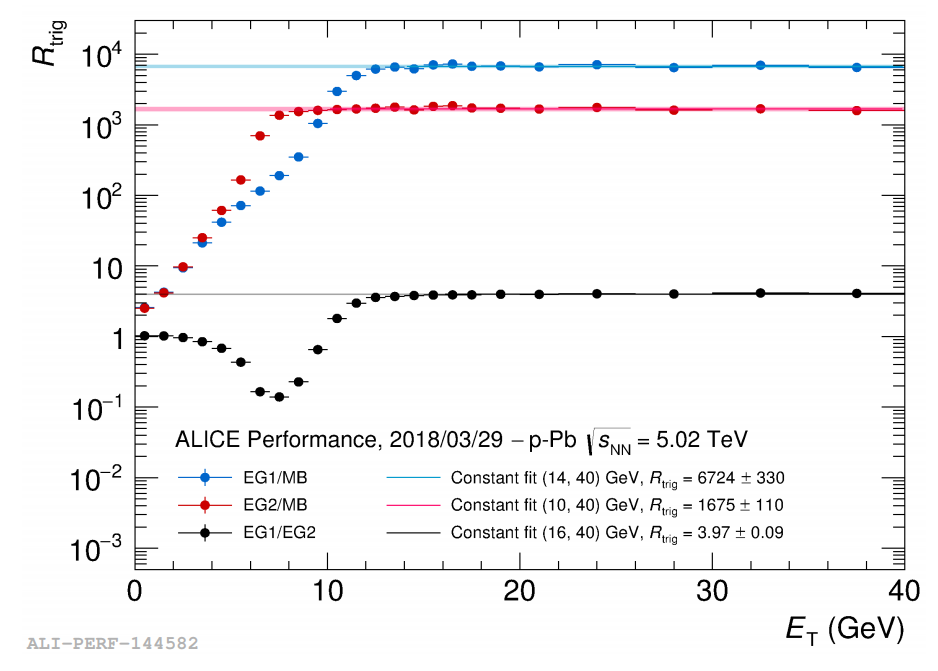
\includegraphics[width=0.6\textwidth]{Datasets/RejectionFactorpPb2013}
%\caption{Rejection factor curves for the 2013 p-Pb period (13def). Source: Ref.~\cite{Erwann}.}
%\label{fig:RejectionFactorpPb}
%\end{figure}


%The total integrated luminosity of the 2013 p-Pb sample is about {4.6 nb$^{-1}$} {($\times$ $A$ = 967 nb$^{-1}$ pp equivalent luminosity)} and about {300 nb$^{-1}$} for the 2017 pp sample. Note that the DCal increases the geometrical acceptance for photons by roughly a factor of 1.3; therefore, comparable statistics of high-$\pt$ photons are expected for pp and p-Pb data.~\footnote{This is the first hard-probes analysis in ALICE that has similar statistics in the reference pp data at the same center-of-mass energy, and thus does not need to rely on extrapolations.}

\begin{table}[h]
   \centering
   \caption{Datasets used in this analysis. The runs listed in the table corresponds to those that are in the good run list appropriate for analysis using the EMCal and ITS detectors.}
   \label{tab:datasets}
   \begin{tabular*}{1.0\columnwidth}{@{\extracolsep{\fill}}llccc@{}}
      	\hline
        Name  & Config. &  Run Number list  & Pass &  Integrated Luminosity\\
        \hline
        %13b& p-Pb & 195344, 195351, 195389, & pass4& $\sim$1.0 nb$^{-1}$\\
        %\hline
      	13d& p-Pb & 195872, 195871, 195867, 195831, 195829,  & pass4& $\sim$1.0 nb$^{-1}$\\
        &  & 195787, 195783, 195767, 195760, 195724. &   &\\
        \hline
        13e & p-Pb & 196310, 196309, 196308, 196214, 196208, & pass4 & $\sim$1.3 nb$^{-1}$\\
         &  &      196201, 196200, 196199, 196197, 196194, & & \\ 
         &  &     196187, 196185, 196107, 196091, 196090, & & \\
         &  &    196089, 196085, 195958, 195955, 195935.  & & \\
         \hline
         13f & Pb-p & 197342, 197341, 197302, 197300, 197299, & pass4 & $\sim$2.3 nb$^{-1}$\\
          &  &                 197298, 197297, 197296, 197260, 197258,&  &\\
          &  &                 197256, 197255, 197254, 197248, 197247,& & \\
          &  &                 197189, 197153, 197152, 197138, 197092,&  &\\
          &  &                 197091, 197027, 197015, 197012, 197011,& & \\
          &  &                 197003, 196974, 196973, 196972, 196967,&  & \\
          &  &                 196965, 196721, 196720, 196714, 196706, & & \\
          &  &                 196703, 196702, 196701, 196648, 196646,& & \\
          &  &                 196608, 196535, 196528. & &\\               \hline

  	17q & pp & 282441, 282440, 282439, 282437, 282415,  & pass1\_wSDD & $\sim$300 nb$^{-1}$\\
     &  & 282411, 282402, 282399, 282398, 282393,  & &\\ 
     & & 282392, 282391, 282367, 282366, 282365  & & \\
		\hline  
   \end{tabular*}
\end{table}

%
%282016, 282008
